\chapter{Konzeption der Megamap-Anwendung}
\label{chap:concept}
Dieses Kapitel beschreibt die Konzeption der im Rahmen dieser Arbeit entwickelten Megamap-Anwendung.
Da in dieser Arbeit die Kartenexploration im Gegensatz zur -navigation stärker fokussiert wird, wird zunächst der Begriff der Kartenexploration definiert.
Um zu verstehen, wie eine digital unterstütze Kartenexploration umgesetzt werden kann, werden Elemente zur Kartenexploration aus bereits existierenden Kartenanwendungen herausgearbeitet.
Diese Elemente werden kategorisiert, zusammengefasst und schließlich als Grundlage für das Megamap-Konzept verwendet.
%Schließlich wird ein Überblick der für die Implementierung benötigten Komponenten gegeben.

\section{Definition Kartenexploration}
\label{sec:definition_exploration}
% Hier die Guidelines einarbeiten
Bereits \textcite{Reichenbacher2001} beschreibt Konzepte zur mobilen Nutzung von digitalen Kartensystemen.
Er gibt eine Übersicht verschiedener \emph{User Tasks}, die in mobilen Umgebungen ausgeführt werden können (siehe \autoref{tab:gis_user_tasks}).
Einer dieser User Tasks ist die \textbf{Navigation}, welcher in digitalen Kartensystemen durch Wegbeschreibungen umgesetzt wird.
Nutzer bekommen einen oder mehrere Pfade zwischen zwei Punkten angezeigt, welche den Nutzern z.B. den schnellsten oder den kürzesten Weg zum Ziel anschaulich machen.
Zusätzlich können wegweisende Textinformationen die Navigation erleichtern.

Neben der Navigation nennt \citeauthor{Reichenbacher2001} drei weitere Kategorien von User Tasks:

\textbf{Lokalisierungs-Tasks (\emph{Locators})} sind Anwendungsfälle, bei denen Nutzer Positionen abfragen und diese angezeigt werden.
Dabei kann es sich um die eigene Position handeln, aber auch um die von anderen Personen oder Objekten.

\textbf{Nähe-Tasks (\emph{Proximity})} sind Anwendungsfälle, bei denen Nutzer Informationen über die Umgebung relativ zur eigenen Position erhalten.
So können Nutzer z.B. die Umgebung nach den nächstgelegenen Geschäften oder Freizeitbeschäftigungen abfragen.

\textbf{Events} sind nicht nur ortsabhängig, sondern auch zeitabhängig.
Bei diesen Anwendungsfällen geht es um die Abfrage von Informationen, die sich mit der Zeit ändern.
Z.B. fallen die Abfrage von geöffneten Geschäften oder von Verkehrsinformationen in diese Kategorie.

Eine Gemeinsamkeit dieser Anwendungsfälle ist, dass hier Informationen über die Umgebung abgefragt werden.
Die Informationen sind abhängig von \emph{mindestens} einem Kontext, zum Beispiel der aktuellen Position der Nutzers.
Es können aber auch mehrere Kontexte gleichzeitig mit einbezogen werden (Beispiel: \enquote{Alle \emph{Geschäfte} in \emph{der Nähe}, die \emph{zurzeit} geöffnet sind} $\rightarrow$ Zweck-, Positions- und Zeitkontext).
Dies steht im Kontrast zur Navigation, für welche immer ein Endpunkt im Kontext zu \emph{mindestens} einem Startpunkt stehen muss (weitere Kontexte wären z.B. Zwischenstopps, das genutzte Fortbewegungsmittel oder das aktuelle Verkehrsaufkommen).

Da Nutzer eine Umgebung durch Abfragen ihrer Informationen \enquote{entdecken}, wird in dieser Arbeit \textbf{Kartenexploration} als Oberbegriff für die Lokalisierungs-, Nähe- und Event-Tasks betrachtet.
Somit grenzt sich die Kartenexploration von der reinen Navigation durch die zuvor beschriebenen Unterschiede ab.

\begin{table}[tbh]
    \centering
    \caption{Geoinformationsaufgaben in einer mobilen Umgebung. \quelle{\cite[47]{Reichenbacher2001}}}
    \label{tab:gis_user_tasks}
    \begin{tabular}{@{}lll@{}}%\toprule
        \tableheadcolor \textsf{\textbf{Tasks}} & \textsf{\textbf{Subtasks}} & \textsf{\textbf{Examples}}\\% \midrule
        \rowcolorodd & Own position & xy coordinates, place name \\
        \rowcolorodd & Objects & Attributes of an object\\
        \rowcolorodd \multirow{-3}{*}{Locators} & Other persons position & Who is this?\\% \midrule
        \rowcoloreven & Objects & Next object with certain attributes\\
        \rowcoloreven \multirow{-2}{*}{Proximity} & Persons & Known people in the area?\\% \midrule
        \rowcolorodd Navigation & Routing & Way descriptions\\% \midrule
        \rowcoloreven Events & What happens at a place & Obstacles (e.g. traffic jam)?\\% \bottomrule
    \end{tabular}
    \vspace{0.5em}
\end{table}

\section{Explorationselemente in existierenden Kartenanwendungen}
\label{sec:exploration_elements}
\todo{Die Texte und Grafiken müssen hier noch etwas fine-tuned werden.}
Digitale Kartenanwendungen setzen unterschiedliche Elemente ein, um die Kartenexploration zu unterstützen.
Bevor das Konzept für die Megamap formuliert wird, werden die Darstellungselemente und Interaktionsmöglichkeiten zur Kartenexploration in bereits existierenden Anwendungen gesammelt und kategorisiert.
Die Idee ist, diejenigen Elemente in der Megamap zu übernehmen, welche Nutzern bereits aus den anderen Anwendungen bekannt sind.
Durch die Verwendung der bekannten Elemente und Interaktionen soll ein zusätzlicher Lernaufwand für die neuartige Megamap-Anwendung verhindert werden.
Die gesammelten Elemente und Interaktionsmöglichkeiten werden jeweils den User Tasks aus \autoref{sec:definition_exploration} zugeordnet.
Demnach ergeben sich drei Kategorien von Explorationselementen: \textbf{Lokalisierungselemente}, \textbf{Nähe-Elemente} und \textbf{Eventelemente}.

Als Beispiele für existierende Kartenanwendungen wurden die \emph{Web}-Varianten von \emph{Google Maps}, \emph{Bing Maps} \parencite{Microsoft2018b} und \emph{HERE WeGo} \parencite{HERE2018} untersucht.
Alle drei Webseiten bieten neben der Routen-Planung auch Funktionen zur Erkundung von Umgebungen an.
\autoref{tab:exploration_elements_summary} zeigt eine Übersicht der gefundenen Explorationselemente.
Die einzelnen Elemente werden in den folgenden Abschnitten mit Beispielen näher erläutert.

\begin{table}[tbh]
    \small
    \centering
    \caption{Übersicht der Explorationselemente in ausgewählten Anwendungen}
    \label{tab:exploration_elements_summary}
    \todo[inline]{TCTD aus Tabelle rausnehmen?}
    \begin{tabular}{@{}lcccc@{}}
        \tableheadcolor \textsf{\textbf{Explorationselement}} & \textsf{\textbf{Google Maps}} & \textsf{\textbf{Bing Maps}} & \textsf{\textbf{Here WeGo}} & \textsf{\textbf{TCTD}}\\

        \tableheadcolor \multicolumn{5}{@{}l@{}}{\textsc{Lokalisierung}} \\
        \rowcolorodd Positionsmarker (Nutzer) & \checkmark & \checkmark & \checkmark & \\
        \rowcoloreven Labels (Straßen, Flüsse, \dots) & \checkmark & \checkmark & \checkmark & \\
        \rowcolorodd Gebäudemarkierungen & \checkmark & \checkmark & \checkmark & \\
        \rowcoloreven Klickmarkierung (Adresse, Koordinaten) & \checkmark & \checkmark & \checkmark & \\
        \rowcolorodd Spezifische Suche (mittels Suchfeld) & \checkmark & \checkmark & \checkmark & \\
        \rowcoloreven Attributsübersicht & \checkmark & \checkmark & --- & \\

        \tableheadcolor \multicolumn{5}{@{}l@{}}{\textsc{Nähe}} \\
        \rowcolorodd Gebäudemarkierungen (Positionsabh.) & \checkmark & \checkmark & \checkmark & \\
        \rowcoloreven Gebäudemarkierungen (Zoomabh.) & \checkmark & \checkmark & \checkmark & \\
        \rowcolorodd Entfernungen (außerhalb Navigation) & \checkmark & \checkmark & --- & \\
        \rowcoloreven Offene Suche (mittels Suchfeld) & \checkmark & \checkmark & \checkmark & \\
        \rowcolorodd Nahbereichssuche & \checkmark & \checkmark & --- & \\
        \rowcoloreven Filter u. Sortierung & \checkmark & \checkmark & --- & \\
        \rowcolorodd Ortsnachbarschaft & \checkmark & \checkmark & Nur Transport & \\
        \rowcoloreven Umgebungsbilder & \checkmark & \checkmark & --- & \\

        \tableheadcolor \multicolumn{5}{@{}l@{}}{\textsc{Event}} \\
        \rowcolorodd Öffnungszeiten & \checkmark & \checkmark & \checkmark & \\
        \rowcoloreven Verkehrsinformationen & \checkmark & \checkmark & \checkmark & \\
        \rowcolorodd Veranstaltungen & \checkmark & --- & --- & \\
        \rowcoloreven Besucheraufkommen & \checkmark & --- & --- & \\

    \end{tabular}
\end{table}

\subsection{Lokalisierungselemente}
\label{ssec:loc-elements}
Lokalisierungselemente sind solche, die wichtige oder interessante Orte auf der Karte markieren.
Die Untersuchung der Beispielanwendungen ergab fünf Arten von Lokalisierungselementen:

Der \emph{Positionsmarker} ist ein grafisches Element auf der Karte, der die aktuelle Position des Nutzer (und unter Umständen auch die Blickrichtung) repräsentiert.
Ein Beispiel findet sich in \autoref{fig:gm_positionsmarker}.
Die Standortdienste des jeweiligen Endgeräts werden benutzt, um den Marker auf der Karte zu platzieren.
Der Positionsmarker erlaubt es dem Nutzer, seine eigene Position in der Umgebung zu bestimmen.

\emph{Labels} sind Textelemente, welche die Namen von Straßen, Flüssen, Gebäuden etc. auf der Karte zeigen (siehe \autoref{fig:hwg_labels}).
Nutzer können Kartenlabels mit Schildern und Wegweisern in der Umgebung abgleichen, was die Orientierung erleichtert.
Zudem sind Wegbeschreibungen deutlicher, wenn Orte auf der Karte und in der Umgebung explizit benannt werden können.
\begin{figure}[h]
    \centering
    \begin{minipage}[t]{.485\textwidth}
        \centering
        \vspace{0pt}
        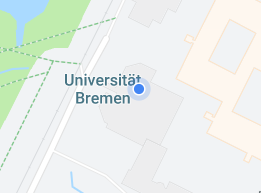
\includegraphics[width=\linewidth, height=4.5cm]{figures/map-app_examples/gm_positionsmarker}
        \captionof{figure}{Beispiel eines Positionsmarkers in Google Maps.}
        \label{fig:gm_positionsmarker}
        \vfill
    \end{minipage}
    \hfill
    \begin{minipage}[t]{.485\textwidth}
        \centering
        \vspace{0pt}
        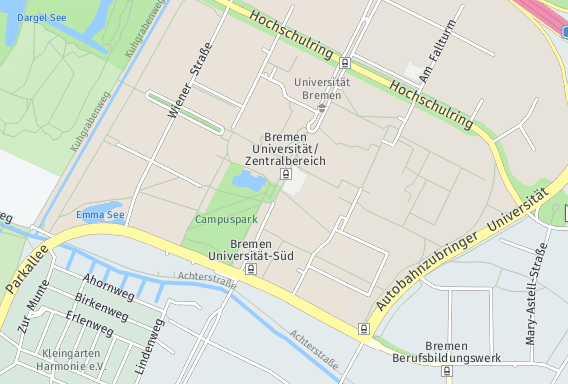
\includegraphics[width=\linewidth, height=4.5cm]{figures/map-app_examples/hwg_labels}
        \captionof{figure}{Beispiel von Labels in HERE WeGo.}
        \label{fig:hwg_labels}
    \end{minipage}
\end{figure}

\emph{Gebäudemarkierungen} sind grafische Elemente, welche die Positionen von gewissen Gebäuden auf Karten markieren.
Es gibt sowohl statische Gebäudemarkierungen, die zusammen mit den Labels auf der Karte fest verankert sind, wie auch dynamische Gebäudemarkierungen, die je nach Kontext des Nutzers ein- bzw. ausgeblendet werden.
Die dynamischen Gebäudemarkierungen werden durch sogenannte \enquote{Stecknadeln} repräsentiert.
Diese sind mit Icons versehen, welche die Kategorie des Gebäudes anzeigen.
Beispiele finden sich in \autoref{fig:bm_gebaeudemarkierungen}.

Eine \emph{Klickmarkierung} kann in den Kartenanwendungen durch Klicken auf den Kartenbereich erzeugt werden.
Die Markierung wird grafisch als Stecknadel oder ein vergleichbares Symbol dargestellt (siehe \autoref{fig:gm_klickmarkierung}).
Über eine solche Markierung kann der Nutzer auf die Adresse und / oder die Koordinaten am angeklickten Ort zugreifen.
\begin{figure}[t]
    \centering
    \begin{minipage}[t]{.485\textwidth}
        \centering
        \vspace{0pt}
        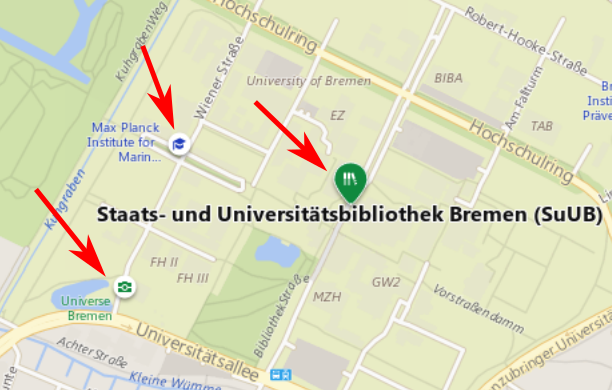
\includegraphics[width=\linewidth, height=4.5cm]{figures/map-app_examples/bm_gebaeudemarkierungen_arrows}
        \captionof{figure}{Beispiel von Gebäudemarkierungen in Bing Maps (hervorgehoben durch \textcolor{red}{rote} Pfeile). %
        Ausgewählte Orte werden durch Stecknadeln stärker betont.}
        \label{fig:bm_gebaeudemarkierungen}
        \vfill
    \end{minipage}
    \hfill
    \begin{minipage}[t]{.485\textwidth}
        \centering
        \vspace{0pt}
        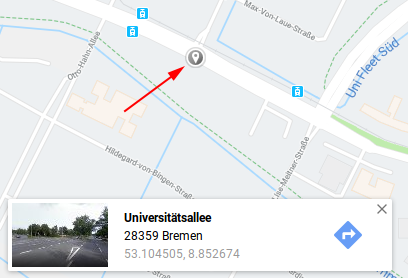
\includegraphics[width=\linewidth, height=4.5cm]{figures/map-app_examples/gm_klickmarkierung}
        \captionof{figure}{Beispiel der Klickmarkierung in Google Maps (hervorgehoben durch \textcolor{red}{roten} Pfeil). %
        Unterhalb der Markierung werden die Adresse und Koordinaten gezeigt.}
        \label{fig:gm_klickmarkierung}
    \end{minipage}
\end{figure}

Die \emph{spezifische Suche} ist eine Lokalisierungs-Interaktion, die durch ein Suchfeld ausgelöst wird.
Als \emph{spezifische} Suche (im Gegensatz zur \emph{offenen} Suche) wird in dieser Arbeit die Suche nach einer bekannten Adresse oder einem eindeutig benannten Ort verstanden (beispielsweise \enquote{Bremer Rathaus} oder \enquote{Bibliothekstraße 1}).
Wird eine solche Suche durchgeführt, platziert die Anwendung eine grafische Markierung auf dem Zielobjekt.
Den Nutzern bleibt somit eine manuelle Suche nach dem Zielort auf der Karte erspart.

Das letzte Lokalisierungselement ist die \emph{Attributsansicht}.
Über diese Ansicht werden Nutzern Informationen über einen Ort aufgelistet.
Die Informationen umfassen neben der Adresse und Anschrift unter anderem auch Kontaktdaten (Webseiten, Telefonnummern), Öffnungszeiten, Bilder, Bewertungen usw.
Speziell für Gebäude werden hier auch Ausstattungen gelistet.
\autoref{fig:gm_ausstattung} zeigt beispielsweise, wie in der Attributansicht von Google Maps die Ausstattung eines Hotels aufgelistet wird.
Die Anzeige solcher Informationen ermöglicht es, die Kartenanwendungen für andere Anwendungsfälle als die reine Navigation zu nutzen.
Dem obigen Beispiel folgend können Nutzer mit der Kartenanwendung ihre Unterkunft während einer Reise planen und werden dann zur Buchung auf die jeweilige Seite des Hotels weitergeleitet.
\begin{figure}[t]
	\centering
	\imagebox{
		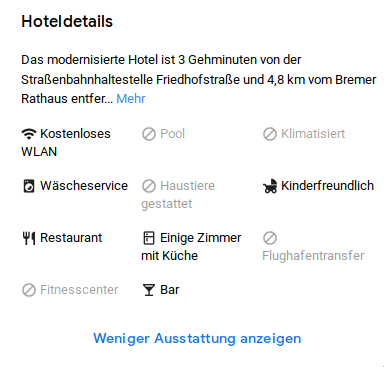
\includegraphics[height=7cm]{figures/map-app_examples/gm_ausstattung}
	}
	\caption{Beispiel für die Auflistung einer Gebäudeausstattung (eines Hotels in Bremen) in der Attributansicht von Google Maps.}
	\label{fig:gm_ausstattung}
\end{figure}

\subsection{Nähe-Elemente}
\label{ssec:prox-elements}
Nähe-Elemente sind Explorationselemente, die im Bezug zur Position des Nutzers stehen und eine Übersicht der näheren Umgebung des Nutzers ermöglichen.
Nutzer können diese Elemente verwenden, um sich ein Bild von der Umgebung zu machen.
Vor allem bei der offenen Suche nach unspezifischen Orten (z.B. \enquote{Restaurants in der Nähe}) kommen die Nähe-Elemente zum Einsatz, indem mehrere Alternativen als Zielorte angeboten werden.
Bei der Untersuchung der Beispielanwendungen ergaben sich acht Arten von Nähe-Elementen:

\emph{Positionsabhängige Gebäudemarkierungen} sind, wie bereits in \autoref{ssec:loc-elements} beschrieben, grafische Elemente, die für den Nutzer interessante oder wichtige Gebäude markieren.
Die Gebäudemarkierungen werden zu einem Nähe-Element, wenn nur die Markierungen in der näheren Umgebung des Nutzers eingeblendet werden.
So können sich Nutzer auf nahegelegene Alternativen konzentrieren und die weiter entfernten Ziele ausblenden.
Erweitert wird dies in den untersuchen Anwendungen durch die \emph{zoomabhängigen Gebäudemarkierungen}.
Hierbei werden Markierungen, die als weniger wichtig für den Nutzer betrachtet werden, erst bei einem hohen Zoom der Karte angezeigt.
Somit können vom Anbieter der Karte zum Beispiel beliebte, häufig frequentierte Ziele hervorgehoben werden, während wenig besuchte Ziele erst später eingeblendet werden.

\emph{Entfernungen} können als Nähe-Elemente außerhalb der reinen Navigation eingesetzt werden, um Nutzern eine konkrete Vorstellung der Umgebung zu erleichtern.
Nutzer können dadurch Reisezeiten abschätzen und bei mehreren Zielalternativen die mit dem kürzesten Reiseweg wählen.
Entfernungen werden zum Beispiel zusammen mit anderen Ortsinformationen angezeigt, oder Nutzer benutzen ein virtuelles Maßband zum Abmessen auf der digitalen Karte.

Die \emph{offene Suche} ist eine Nähe-Interaktion, die über ein Suchfeld ausgelöst wird.
Anders als die \emph{spezifische} Suche wird bei der offenen Suche nach Kategorien von Orten gesucht (z.B. \enquote{Restaurants}, \enquote{Parks}, \enquote{Zoo}).
Da bei einer solchen offenen Suche keine eindeutigen Ortsnamen verwendet werden, kommt es häufig zu mehreren Zielalternativen, die für die Nutzer zutreffen könnten.
In den untersuchten Anwendungen werden alle möglichen Alternativen durch Gebäudemarkierungen hervorgehoben.
\autoref{fig:bm_open_search} zeigt eine offene Suche nach Hotels in Bremen.
\begin{figure}[h]
	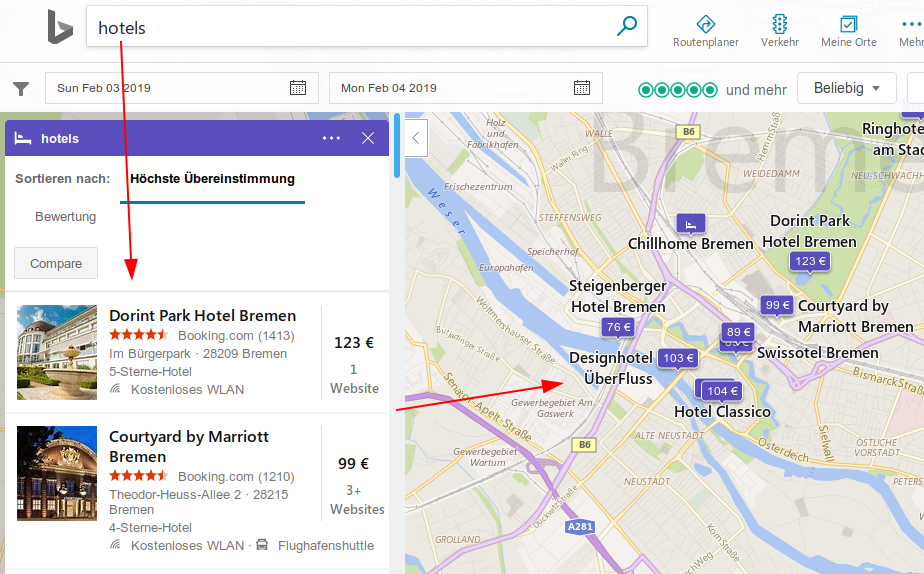
\includegraphics[width=\linewidth]{figures/map-app_examples/bm_open_search_2}
	\caption{Offene Suche nach Hotels in Bing Maps liefert mehrere Alternativen.}
	\label{fig:bm_open_search}
\end{figure}

Die \emph{Nahbereichssuche} ist eine Interaktion, mit der ein definierter Bereich der Karte unter Suchkriterien nach Orten durchsucht werden kann.
Damit ist sie eine lokal begrenzte offene Suche.
In den untersuchten Anwendungen lässt sich diese Funktion durch Öffnen des Kartenmenus mittels Rechtsklick aufrufen (siehe \autoref{fig:bm_nearby}).
Bei der Nahbereichssuche werden nur Gebäudemarkierungen angezeigt, die sich in einem gewissen Radius um den Ort des Anklickens herum befinden.
Nutzer können hiermit Umgebungen erkunden, an denen sie sich selber nicht befinden.

Über die Elemente \emph{Filter und Sortierung} können die Suchkriterien weiter eingeschränkt werden.
Beispielsweise lassen sich Restaurants nach der gewünschten Küche filtern, oder Hotels nach Preisklasse (siehe \autoref{fig:bm_sorting}).
So müssen Nutzer nicht sämtliche verfügbare Alternativen per Hand durchgehen, um zu prüfen, ob die Alternativen ihren Vorstellungen entsprechen.
Die Filterung und Sortierung kann Nutzern somit durch das Ausblenden irrelevanter Orte Zeit beim Suchen von Zielen ersparen.

\begin{figure}[p]
    \centering
    \imagebox{
	    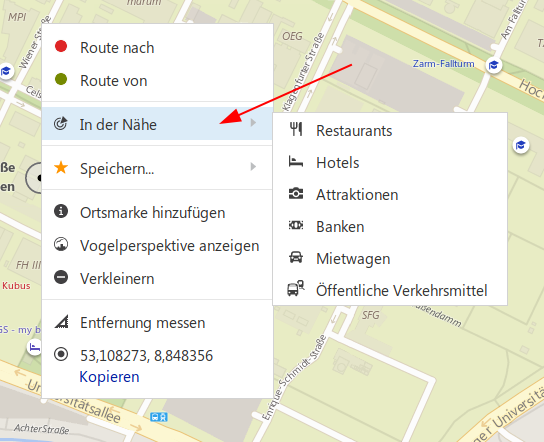
\includegraphics[width=0.485\linewidth]{figures/map-app_examples/bm_nearby}
	}
	\caption{Über das Rechtsklick-Menu in Bing Maps kann die Umgebung durchsucht werden.}
	\label{fig:bm_nearby}
\end{figure}
\begin{figure}[p]
	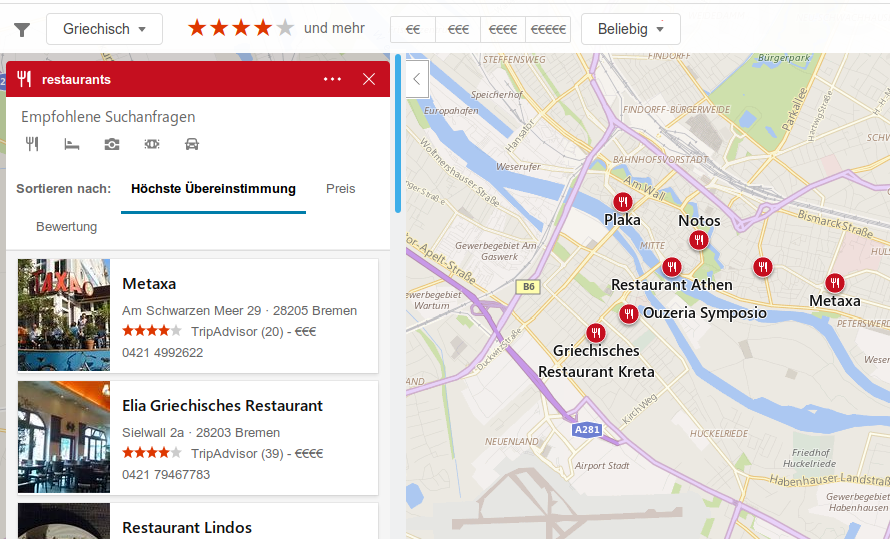
\includegraphics[width=\linewidth]{figures/map-app_examples/bm_filter_sorting}
	\caption{Anzeige und Sortierung von griechischen Restaurants mit einer 4-Sterne-Bewertung oder höher (in Bing Maps).}
	\label{fig:bm_sorting}
\end{figure}

Das Nähe-Element \emph{Ortsnachbarschaft} ist ein Element, welches in der Ansicht über die Ortsinformationen integriert sein kann.
Hierbei handelt es sich um eine List von weiteren Orten, die für den Nutzer relevant sein könnten und sich in der Nähe des aktuell betrachteten Orts befinden.
Auch die Information über nahegelegene Transportmöglichkeiten fällt unter diese Kategorie.

Schließlich finden sich \emph{Umgebungsbilder} in den Kartenanwendungen als Nähe-Element.
Sie zeigen Foto-Aufnahmen (gegebenenfalls als 360\textdegree-Aufnahme) der Umgebung.
Wie die Gebäudemarkierungen sind die abgebildeten Orte auf einen gewissen Radius um einen Ausgangspunkt herum beschränkt, sodass für die Nutzer irrelevante Bilder nicht gezeigt werden.
Die Einbindung der Bilder in die Anwendungen wird unterschiedlich gehandhabt.
Zum Beispiel befindet sich in Google Maps eine Liste von Umgebungsfotos in Attributsansicht.
Wird die Liste angeklickt, öffnet sich eine Großansicht der Fotos (siehe \autoref{fig:gm_photos}).
Handelt es sich bei dem Bild um eine 360\textdegree-Aufnahme, kann mit der Maus die Ansicht verändert werden.
\begin{figure}[h]
	\centering
	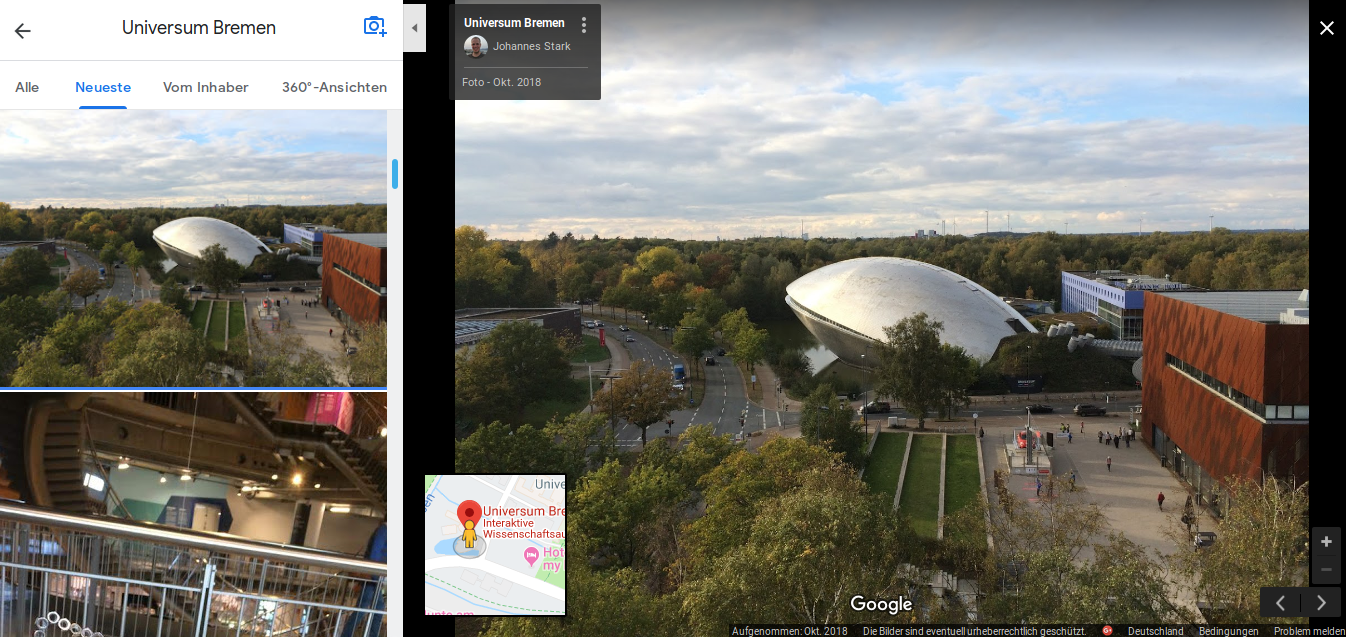
\includegraphics[width=\linewidth]{figures/map-app_examples/gm_photos_2}
	\caption{Umgebungsfotos zum Universum Bremen via Google Maps.}
	\label{fig:gm_photos}
\end{figure}

\subsection{Event-Elemente}
\label{ssec:event-elements}
Event-Elemente integrieren zeitliche Geschehnisse in die digitalen Karten.
Die Eventinformationen werden live aus diversen Datenquellen bezogen, wodurch die Karten in Echtzeit aktualisiert werden.
Bei der Untersuchung der Beispielanwendungen ergaben sich vier Arten von Event-Elementen:

Die \emph{Verkehrsinformationen} informieren Nutzer über die aktuelle Situation des Straßenverkehrs.
Verkehrsaufkommen, Baustellen, Staus und Umleitungen werden in Echtzeit in die Karten integriert und visualisiert.
Neben der aktuellen Verkehrssituation werden auch Durchschnittswerte für die Befahrung von Straßen angezeigt, sodass Nutzer bereits vorab den Verkehr in der Umgebung abschätzen können

Die \emph{Veranstaltungsinformationen} sind in die Ortsinformationen integriert.
Hier werden die Veranstaltungen der nächsten Tage präsentiert (z.B. Konzerte).
Unter Umständen werden auch die Ticketverfügbarkeit und -preise angezeigt.

\emph{Öffnungszeiten} informieren Nutzer über den Zugang zu Orten in der Umgebung, vor allem Gebäuden.
Dank der Integration der Öffnungszeiten müssen Nutzer nicht weitere Informationen abrufen, um zu schauen, ob das Ziel zur aktuellen Zeit erreicht werden kann.
Wie \autoref{fig:gm_opening_hours} zeigt sind beispielsweise die Öffnungszeiten in Google Maps in der Attributsansicht zu finden.

Zuletzt sind auch Informationen über das \emph{aktuelle Besucheraufkommen an Orten} als Event-Element verfügbar.
Nutzer können zum Beispiel einsehen, ob ein großer Andrang auf ein Geschäft besteht und so lange Wartezeiten beim Schlangestehen vermeiden (siehe \autoref{fig:gm_opening_hours}).
\begin{figure}[th]
	\centering
	\imagebox{
		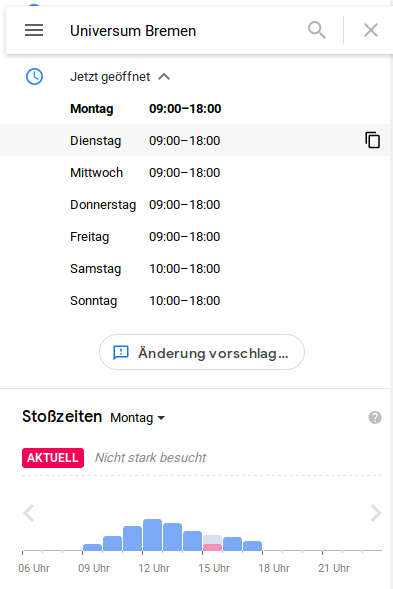
\includegraphics[width=0.4\linewidth]{figures/map-app_examples/gm_opening_hours}
	}
	\caption{Öffnungszeiten von Geschäften etc. werden in Google Maps in der Attributsansicht gezeigt.}
	\label{fig:gm_opening_hours}
\end{figure}

\section{Megamap in \emph{Tom Clancy's The Division}}
% Mechanics

\section{Anwendung der Explorationselemente für Megamap}
Basierend auf den Erkenntnissen der vorigen Abschnitte kann ein Konzept für eine umgebungsintegrierte Megamap entwickelt werden, deren Zielplattform Mixed-Reality-HMDs sind.

\subsection{Nutzungsszenario}
Die Megamap als eine dreidimensionale Karte für MR-HMDs konzipiert.
Vor dem Hintergrund der Umgebung des Nutzers zeigt sie ein dreidimensionales Innenmodell des Gebäudes, in dem sich der Nutzer zur Zeit befindet.
Die Karte wird durch das HMD in die Umgebung des Nutzers integriert.
Vor allem bleibt ihre Rotation in der Umgebung verankert, wenn der Nutzer sich bewegt.
Somit erscheint es, als würde die 3D-Karte tatsächlich in der Umgebung stehen.
Für mehrstöckige Gebäude wird nur das aktuelle Stockwerk angezeigt, wobei Nutzer die Möglichkeit zum Wechsel der Stockwerke haben.
Über Interaktionselemente ist es möglich, Informationen zu Räumen und Objekten auf der Karte abzurufen.
Die Konzeptzeichnung in \autoref{fig:concept_overview} verdeutlicht das Prinzip.

Die Megamap soll Nutzern helfen, sich in unbekannten Gebäuden zu orientieren, diese zu erkunden und nach Orten in den Gebäuden zu suchen.
Ein Beispiel ist die augmentierte Exploration der Gebäude der Universität Bremen.
Neue Studierende oder Gäste der Universität könnten durch die Megamap bei der Suche nach Büros von Mitarbeitern, öffentlichen Druckern, Essensmöglichkeiten, Toiletten etc. unterstützt werden.
Da die meisten der Universitätsgebäude mehrstöckig sind, wäre der Einsatz einer dreidimensionalen Karte zur Exploration der Gebäude interessant.
Auch der Einsatz in Einkaufszentren oder Flughäfen ist denkbar.
\begin{figure}[bht]
	\centering
	\imagebox{
		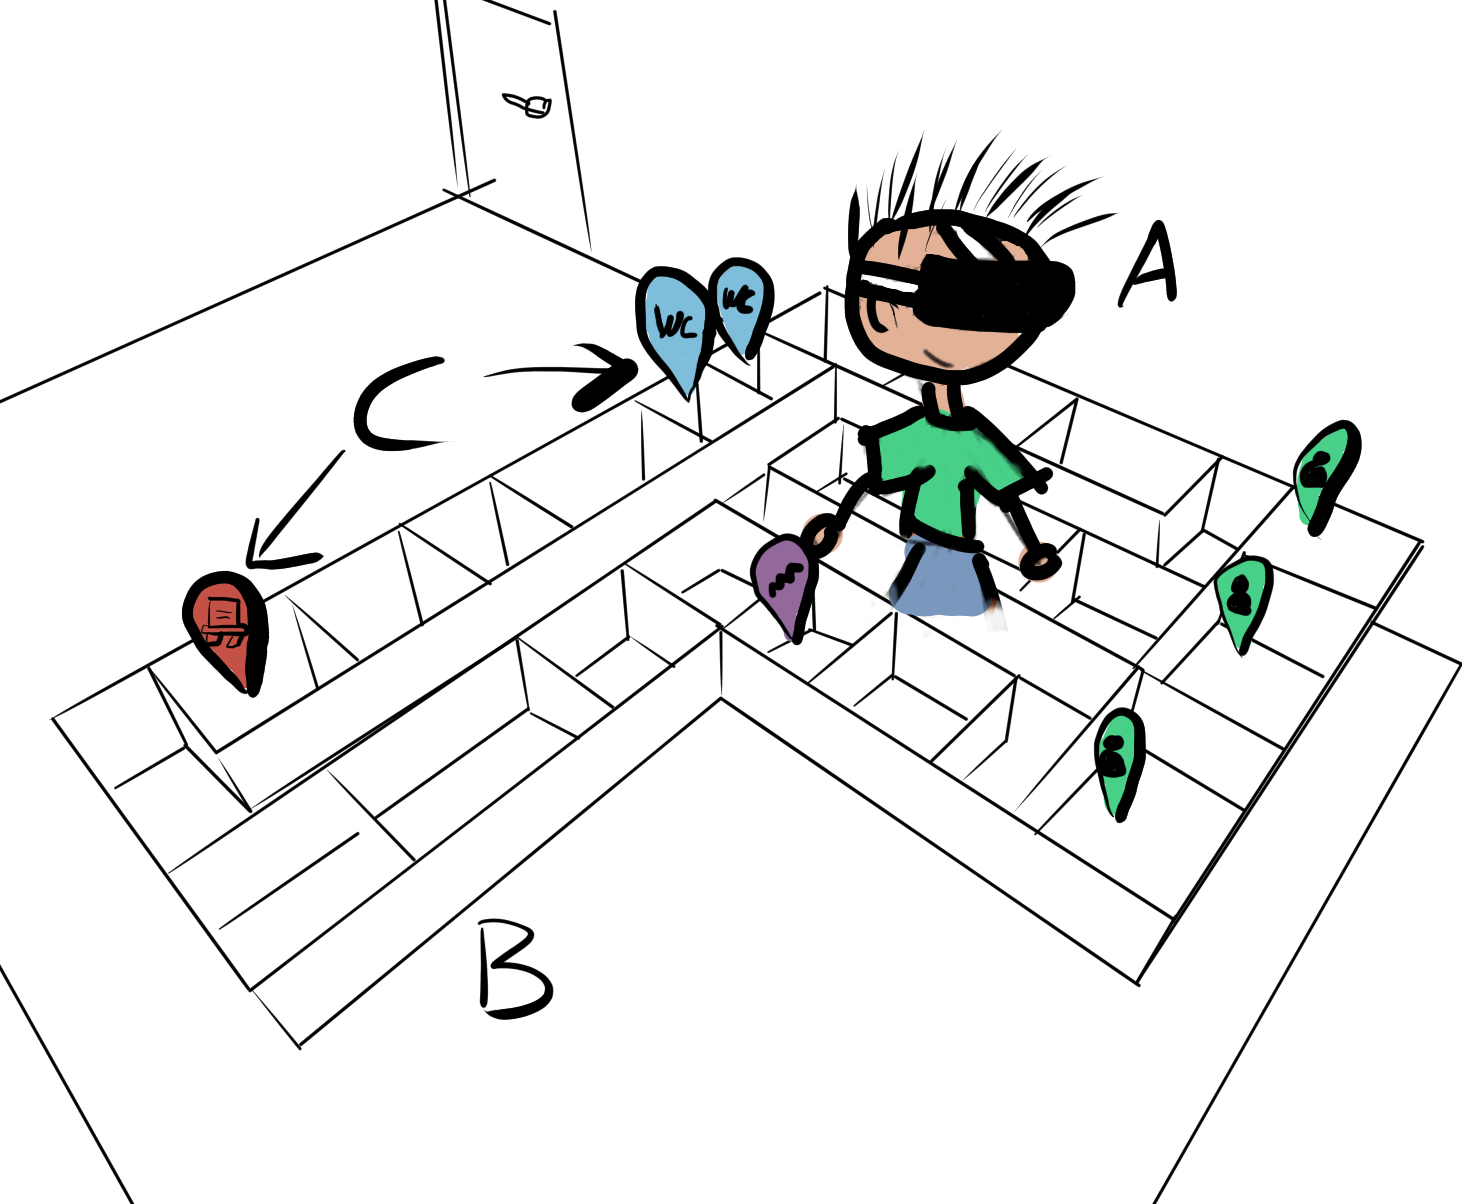
\includegraphics[width=0.75\linewidth]{figures/concept/overview}
	}
	\caption{Konzeptzeichnung einer Megamap. %
		A:~Nutzer trägt ein HMD. %
		B:~Indoor-Megamap wird in Umgebung des Nutzers angezeigt. %
		C:~Stecknadel-Icons markieren Räume mit Kategorien.}
	\label{fig:concept_overview}
\end{figure}

\subsection{Interaktion durch Explorationselemente}
\todo{Kon\-zept\-zeich\-nun\-gen überarbeiten.}
Nutzern von MR-HMDs wie der HoloLens oder der Magic~Leap stehen drei Eingabemethoden zur Verfügung: Controller, Gesten- und Sprachsteuerung.
Da die Megamap in dieser Arbeit als Prototyp in VR implementiert wird, konzentriert sich das Konzept auf die Controller-Methode.

Damit das 3D-Gebäudemodell überhaupt als Karte fungieren kann, müssen Nutzer mit dem Modell interagieren können.
Speziell muss die Karte Explorationselemente anbieten, mit denen Nutzer die Umgebung erkunden können.
Mögliche Explorationselemente sind in \autoref{sec:exploration_elements} beschrieben.
Für das entwickelte Konzept sowie den Prototypen wurde eine kleinere Auswahl der Elemente betrachtet.
Ein Ziel für zukünftige Arbeiten kann daher sein, dass die Megamap die gleiche Zahl an Explorationselementen unterstützt wie herkömmliche 2D-Kartenanwendungen.

Für die Indoor-Megamap werden die Gebäudemarkierungen als \emph{Raum}markierungen umfunktioniert, da bei der Anwendung nur ein Gebäude zur Zeit im Fokus steht.
Die Raummarkierungen werden als dreidimensionale Stecknadeln über Räumen mit besonderen Funktionen dargestellt.
So können interessante Orte im Gebäude hervorgehoben werden.
Durch Icons auf den Stecknadeln kann die Kategorie des Raums hervorgehoben werden (beispielsweise Büro, Toilette etc.).
Ebenso können mit den Stecknadeln wichtige Objekte im Gebäude markiert werden (Drucker, Treppen und Aufzüge, Erste-Hilfe-Kästen etc.).
Über Filterelemente neben der Karte ließen sich dann Stecknadeln einer Art herausfiltern.
Die Konzeptzeichnung in \autoref{fig:concept_indoor_view} zeigt die Indoor-Megamap der Ebene 5 des MZH an der Universität Bremen.
Über eine virtuelle Filterbox werden nur Stecknadeln für öffentliche Toiletten gezeigt.
Stecknadeln werden auch über Stockwerke hinweg angedeutet, indem sie vertikal versetzt und transparent gemacht werden.
So können Nutzer auch Orte und Objekte finden, die auf dem aktuellen Stockwerk nicht vorhanden sind.
\vfill
\begin{figure}[h]
	\centering
	\imagebox{
		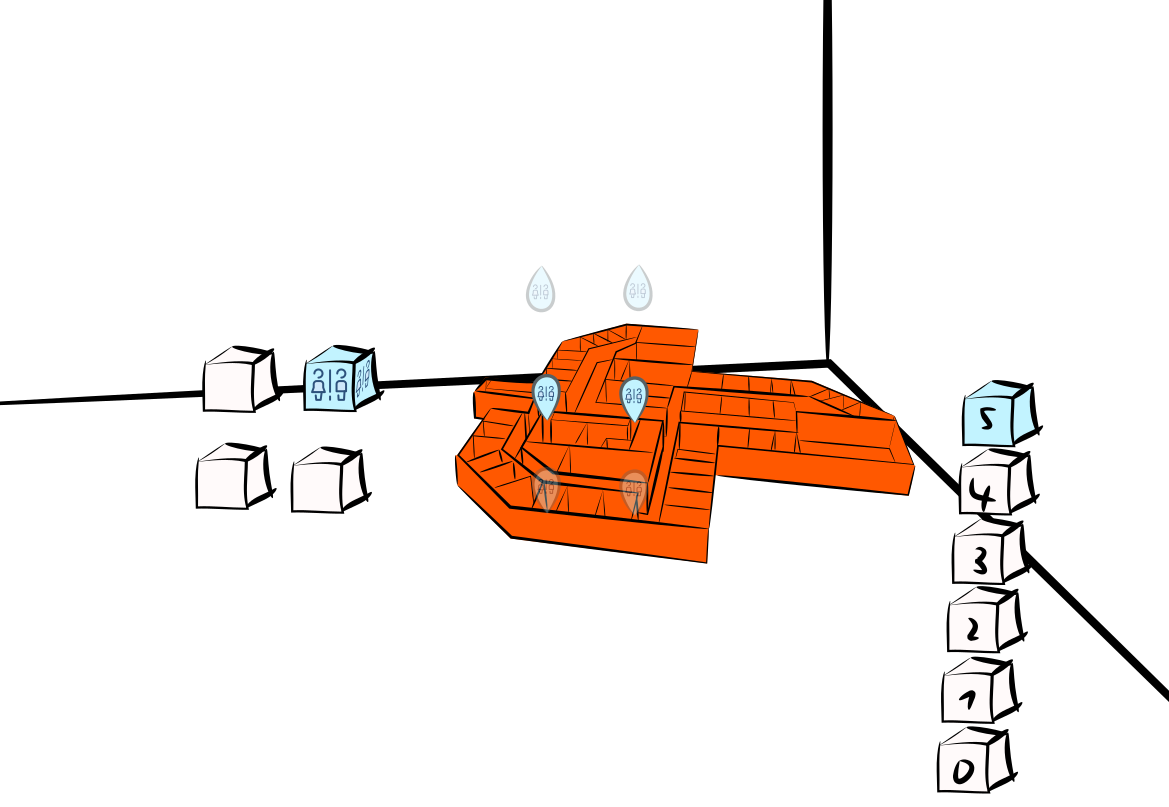
\includegraphics[trim={4cm, 0, 3cm, 5cm}, clip, width=0.7\linewidth]{figures/concept/3d_condition}
	}
	\caption{Konzeptzeichnung Megamap für Stockwerkwechsel, Filter und Suche.}
	\label{fig:concept_indoor_view}
\end{figure}

\newpage
Um mehr Informationen zu einem Ort oder Objekt zu erhalten, können Nutzer die Stecknadel entweder mit dem im Raum getrackten Controller berühren, oder sie mit einem virtuellen Laserpointer anvisieren.
Letztere Variante hat den Vorteil, dass sich Nutzer nicht zu weiter entfernten Stecknadeln hinbewegen müssen.
An der Position des Pins öffnet sich ein Fenster mit Informationen zum Ort bzw. Objekt, was die Aufgabe der Attributsliste aus \autoref{sec:exploration_elements} übernimmt.
Ein Beispiel für ein solches Informationsfenster ist in \autoref{fig:concept_pin_info} skizziert.
Wie die Karte und die Stecknadeln ist auch das Informationsfenster in der Umgebung verankert.
Anstatt es direkt auf dem Display des Nutzers anzuzeigen befindet sich das Fenster an der Position der Stecknadel und wird so rotiert, dass der Nutzer immer auf die Vorderseite schaut.
Seine relative Position zur Umgebung bleibt gleich.
Eine Integration von 2D-Elementen als 3D-Objekt in die Umgebung (anstatt fester Anzeige auf dem Display) verhindert Unwohlsein bei Nutzern sowie eine Verdeckung der Umgebung und anderer virtueller Inhalte \parencite[23]{Schroeder2017}.

Damit Nutzer das aktuell gezeigte Stockwerk wechseln können, ohne sich physisch dorthin zu bewegen, werden weitere virtuelle Schaltflächen angeboten (siehe \autoref{fig:concept_indoor_view}).
Mit diesen kann auf die gleiche Weise wie mit den Stecknadeln oder den Filterelementen über den Controller interagiert werden.

Damit Nutzer ihre Position auf der Karte schnell erkennen können wird der Positionsmarker als Lokalisierungselement für die Megamap übernommen.
Für die Anwendung auf einer 3D-Karte wird der Marker von einem zweidimensionalen Kreis zu einem Zylinder erweitert.
Zusätzlich zeigt ein Kreissegment die aktuelle Blickrichtung sowie den Blickwinkel des Nutzers an.
Somit können Nutzer nicht nur ihre Position, sondern auch ihre Orientierung innerhalb der Umgebung vom Positionsmarker ablesen.

\begin{figure}[bth]
	\centering
	\imagebox{
		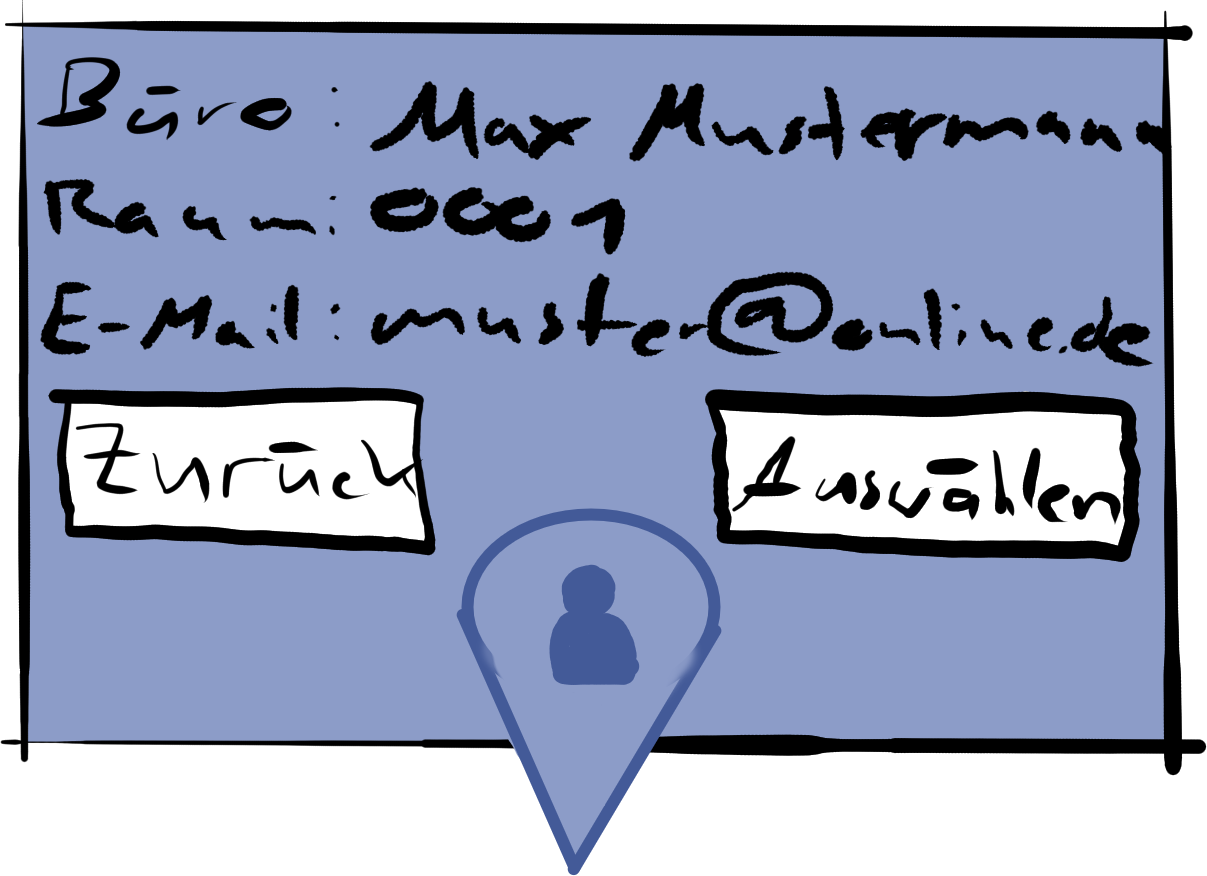
\includegraphics[width=0.72\linewidth]{figures/concept/concept_location_info}
	}
	\caption{Konzeptzeichnung der Stecknadel-Informationen.}
	\label{fig:concept_pin_info}
\end{figure}

\subsection{Platzierung der Megamap im Raum}
Um die Megamap wie ein \enquote{reales} Objekt im Raum zu platzieren wird die 3D-Rekonstruktion des HMDs eingesetzt.
Durch die Rekonstruktion liefert das HMD 3D-Meshes des Bodens, der Wände und vereinfachte Meshes von Objekten der Umgebung.
Die Megamap kann auf dem Boden-Mesh platziert werden, sodass sie in der realen Umgebung ebenfalls auf dem Boden steht.
Durch einen Abstand zum Boden-Mesh wirkt es, als würde die Megamap im Raum schweben.

Analog zur Karte aus TCTD soll die Megamap so um den Nutzer herum platziert werden, dass die Position des Nutzers auf der Karte mit seiner aktuellen Position übereinstimmt.
Das bedeutet, dass zu Beginn (beim Aufrufen der Karte) der Nutzer auf seiner eigenen Markierung steht.
Dies soll Nutzern eine schnellere Orientierung ermöglichen, da sie ihre Position auf der Karte nicht erst wiederfinden müssen.
Damit die Position der Nutzer bestimmt werden kann ist ein System zur Indoor-Lokalisierung erforderlich.
Mehrere Ansätze werden in der Literatur diskutiert, darunter \wifi-Fingerprinting \parencites{Lautenschlaeger2012}{Alnabhan2014}, Magnetfeld-Fingerprinting \parencites{Hashish2017}{Ang2018} oder Bild-basierte Verfahren \parencites{Kalkusch2002}{Moeller2014}{Silva2015}.
Weiterhin könnten die vom HMD gelieferten 3D-Meshes mit vorgefertigten Raummodellen abgeglichen werden, um den aktuellen Raum sowie die aktuelle Position des Nutzers zu bestimmen.

Ein Problem, was bei der Platzierung der virtuellen Karte in die reale Umgebung auftritt, ist die Verdeckung realer Objekte.
Durch eine Verdeckung, bei der Teile des realen Objekts noch sichtbar sind, entsteht eine Störung des Tiefeneindrucks des Nutzers, wodurch der Effekt einer integrierten Karte verloren geht.
TCTD löst das Problem der Verdeckung von Umgebungsobjekten, indem die Karte an den Schnittpunkten mit den Objekten immer weiter ausgeblendet wird, bis schließlich nur noch die Objekte zu sehen sind.
Die Karte wird effektiv an den Objekten \enquote{ausgeschnitten}.
Mit den erwähnten MR-HMDs ist ein solcher Effekt ebenfalls möglich.
Durch die 3D-Rekonstruktion ergeben sich grobe Meshes der Umgebungsobjekte und Wände.
Die virtuelle Megamap kann an den Stellen dieser Meshes transparent gerendert werden, wodurch der Effekt aus TCTD nachgestellt wird.

\subsection{Beschaffung von Gebäudedaten und Generierung der Karten}
Für die Darstellung als Megamap ist ein 3D-Modell des Gebäudes erforderlich.
Eine automatisierte Generierung des Modells basierend auf Gebäudedaten ist wünschenswert, damit das Modell nicht per Hand erstellt werden muss und immer die aktuellsten Daten des Gebäudes nutzt.
Ein möglicher Ansatz ist, die Grundrisse des jeweiligen Gebäudes zu georeferenzieren und in einer entsprechenden Datenbank wie z.B. OpenStreetMap zu veröffentlichen.
Die Megamap-Anwendung kann auf die georeferenzierten Grundriss-Daten über die Programmierschnittstelle (\emph{Application Programming Interface} (API)) zugreifen und daraus 3D-Modelle generieren.
Die Wände des Gebäudes können z.B. als Polygon-Features mit dem OSM-Tag \lstinline{height} angelegt werden, die Türen würden durch Rechtecke mit dem Tag \lstinline{min_height} repräsentiert.
Normalerweise werden in OSM mit diesen Tags Gebäude als Ganzes definiert \parencite{OpenStreetMapFoundation2018b}.
Dennoch lassen sich die Tags für die Definition eines Indoor-Layouts umfunktionieren.

Ergänzend hierzu unterstützt OSM das \emph{Simple Indoor Tagging Schema}.
\autoref{fig:osm_simple-indoor-tagging} zeigt, wie das Schema auf ein Gebäudelayout angewendet werden kann.
Da dieses Schema zum regulären Tagging in OSM kompatibel ist, können Indoor- und Outdoor-Daten in der selben Datenbank verwaltet werden \parencite{OpenStreetMapFoundation2018c}.
\begin{figure}[t]
    \centering
    \imagebox {
        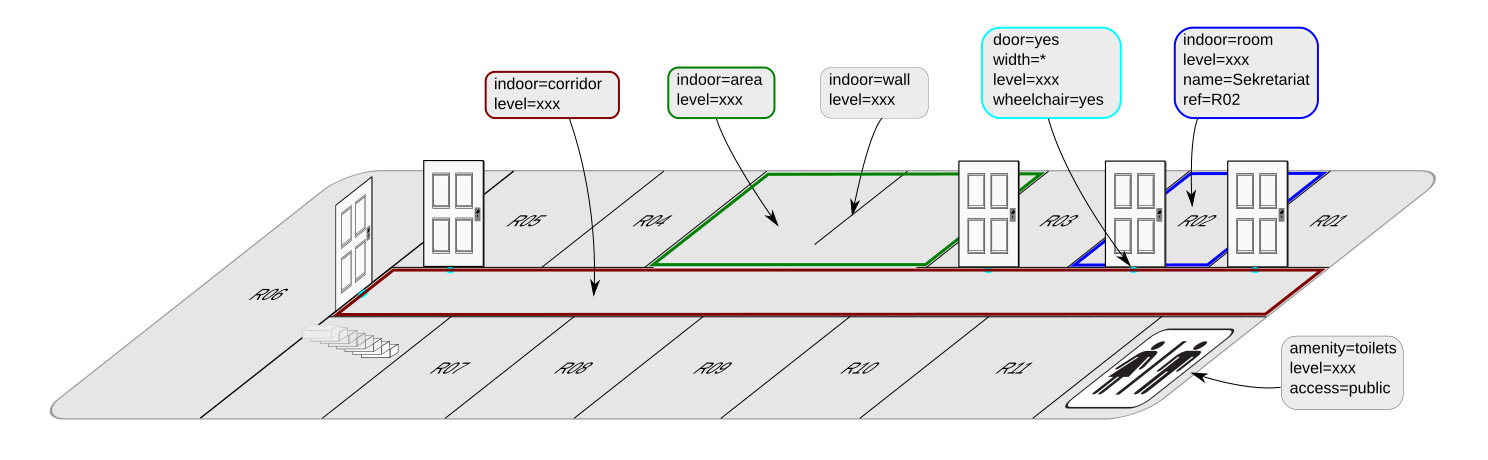
\includegraphics[trim={17cm, 0, 0, 0}, clip, width=\linewidth]{figures/concept/osm_Indoor2_0_elements}
    }
    \caption{Beispiel des Simple Indoor Tagging Schemas in OpenStreetMap. %
    \quelle{\cite{OpenStreetMapFoundation2018c}, Ausschnitt durch Verfasser}}
    \label{fig:osm_simple-indoor-tagging}
\end{figure}

Konkrete Möglichkeiten, die Daten aus OSM abzurufen und für die Megamap zu verwenden, werden in \autoref{chap:closing} diskutiert.
%
\cleardoublepage
